%!TEX program = xelatex
%%%%%%%%%%%%%%%%%%%%%%%这是导言部分的开始%%%%%%%%

%========= 导言部分声明文档的类型=================
\documentclass{article}

	%=========导言部分可可以加载宏包=================
	\usepackage{amsmath}                % 数学公式排版宏包
	\usepackage{amssymb}                % 数学符号命令宏包
	\usepackage{amsthm}                 % 数学定理宏包
	\usepackage[UTF8]{ctex}             % 中文输入宏包
	\usepackage[a4paper]{geometry}      % 页面设置宏包
	\usepackage{setspace}               % 行间距宏包
	\usepackage{graphicx}               % 图片宏包
	\usepackage{listings}               % 代码宏包
	\usepackage{color}					% 颜色宏包
	\usepackage{xcolor}                 % 颜色处理宏包
	\usepackage{float}                  % 浮动对象式样宏包
	\usepackage{fontspec}
	\usepackage{enumerate}				% 列举编号包
	
	%=========页面设置==============================
	\geometry{left=1cm,right=1cm,top=1cm,bottom=2cm}
	\onehalfspacing
	\setlength\parindent{0em}

	%=========代码格式设置============================
	\definecolor{dkgreen}{rgb}{0,0.6,0}
	\definecolor{gray}{rgb}{0.5,0.5,0.5}
	\definecolor{mauve}{rgb}{0.58,0,0.82}
	% \setmonofont{Consolas}
	\lstset{
		numbers = left, 	
		numberstyle = \color{gray}, 
		keywordstyle = \color{blue},
		commentstyle = \color{dkgreen}, 
		stringstyle = \color{mauve},
		basicstyle = \ttfamily,
		breaklines = true,
		frame = shadowbox, % 阴影效果
		rulesepcolor = \color{ red!20!green!20!blue!20} ,
		escapeinside = ``, % 英文分号中可写入中文
		xleftmargin = 2em,xrightmargin=2em, aboveskip=1em,
		framexleftmargin = 2em
	} 

%=========导言部分可以定义标题信息===============
\title{组会报告}
\author{徐益}
\date{\today}
%%%%%%%%%%%%%%%%%%%%%%%这是导言部分的结束%%%%%%%%%

%%%%%%%%%%%%%%%%%%%%%%%这是正文部分的开始%%%%%%%%%
\begin{document}

%=========生成标题================================
\maketitle

%=========开始正文的输入==========================

%===========第一节=================
\section{工作内容}
1. 使用avx2指令实现限幅部分;

2. 完成代码基于linux平台的调试;

3. 在服务器上对译码模块进行性能测试。

%===========第一节=================
\section{使用avx2指令实现限幅部分}
\subsection{使用packs相关指令}
原模块:
\lstset{language=C++}
\begin{lstlisting}
for (r = 0; r < C; r++)
	for (n = 0; n < Nd / 8; n++)
	{
		resf = _mm256_mul_ps(*p_tabI, fact);
		resf = _mm256_max_ps(resf, vminf);
		resf = _mm256_min_ps(resf, vmaxf);
		resi = _mm256_cvttps_epi32(resf);
		p_tabI += 1;
		for (i = 0; i < 8; i++)
			ptr_llr[32 * (8 * n + i) + r] = (int8_t)p_resi[i];
	}
\end{lstlisting}
现模块:
\lstset{language=C++}
\begin{lstlisting}
for (n = 0; n < Nd; n++)
{
	for (i = 0; i < 4; i++)
	{
		vllrf = _mm256_load_ps((float *)p_tabI);
		resf = _mm256_mul_ps(vllrf, fact);
		resf = _mm256_max_ps(resf, vminf);
		resf = _mm256_min_ps(resf, vmaxf);
		resi[i] = _mm256_cvttps_epi32(resf);
		p_tabI += 1;
	}
	vtemp16[0] = _mm256_packs_epi32(resi[0], resi[1]);
	vtemp16[1] = _mm256_packs_epi32(resi[2], resi[3]);
	vtemp8 = _mm256_packs_epi16(vtemp16[0], vtemp16[1]);
	_mm256_store_si256(p_tabO, vtemp8);
	p_tabO++;
}
uchar_transpose_avx(tabO, h->llr_avx2, Nd);
\end{lstlisting}

\subsection{遇到的问题}
\begin{figure}[H]
	\centering
	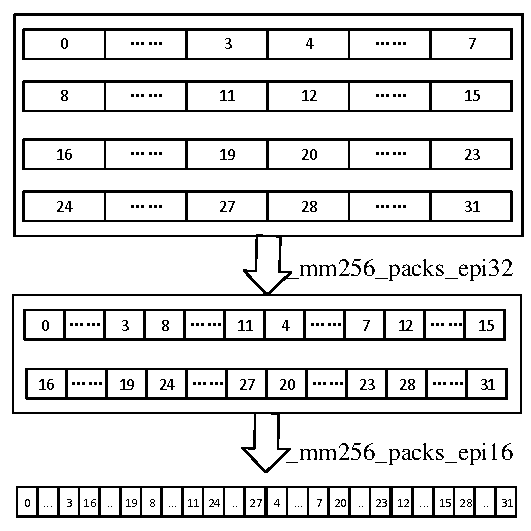
\includegraphics[width = .7\textwidth]{packs.pdf}
	\caption{packs相关指令的过程}
\end{figure}
\begin{figure}[H]
	\centering
	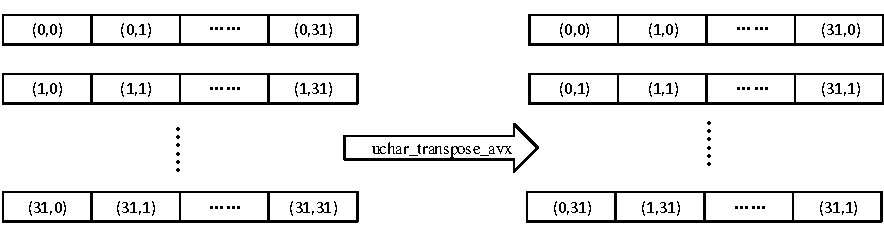
\includegraphics[width = \textwidth]{unpack.pdf}
	\caption{uchar\_transpose\_avx函数的过程}
\end{figure}

%===========第二节=================
\section{代码基于linux平台的调试}
\subsection{遇到的问题}
\begin{figure}[H]
	\centering
	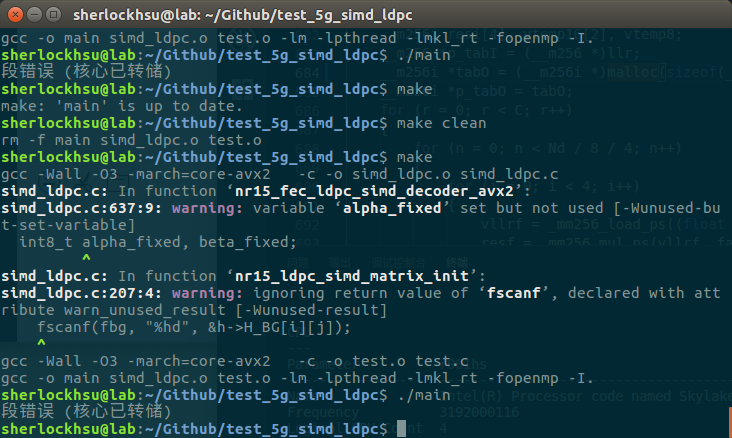
\includegraphics[width = .8\textwidth]{err.png}
	\caption{段错误}
\end{figure}
错误原因:\\
使用malloc函数分配空间时,未对齐寄存器变量地址。\\
解决方法:\\
使用\_mm\_malloc函数分配寄存器相关地址空间;\\
使用\_mm\_free释放相关地址空间。

%===========第三节=================
\section{Linux平台上的性能测试}
\subsection{Linux平台上的VTune测试方法}
1. source /opt/intel/vtune\_amplifier/amplxe-vars.sh\\
2. amplxe-cl -collect hotspots ./main\\
3. amplxe-cl -report hotspots r000hs
\subsection{本地测试}
\begin{figure}[H]
	\centering
	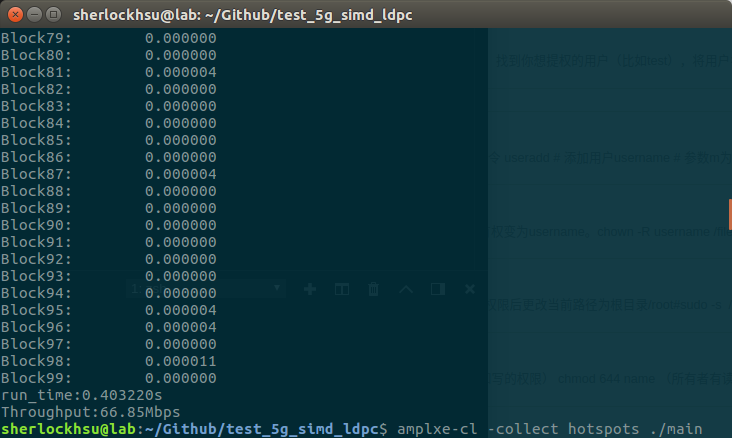
\includegraphics[width = .8\textwidth]{resl.png}
	\caption{本地运行结果}
\end{figure}
\begin{figure}[H]
	\centering
	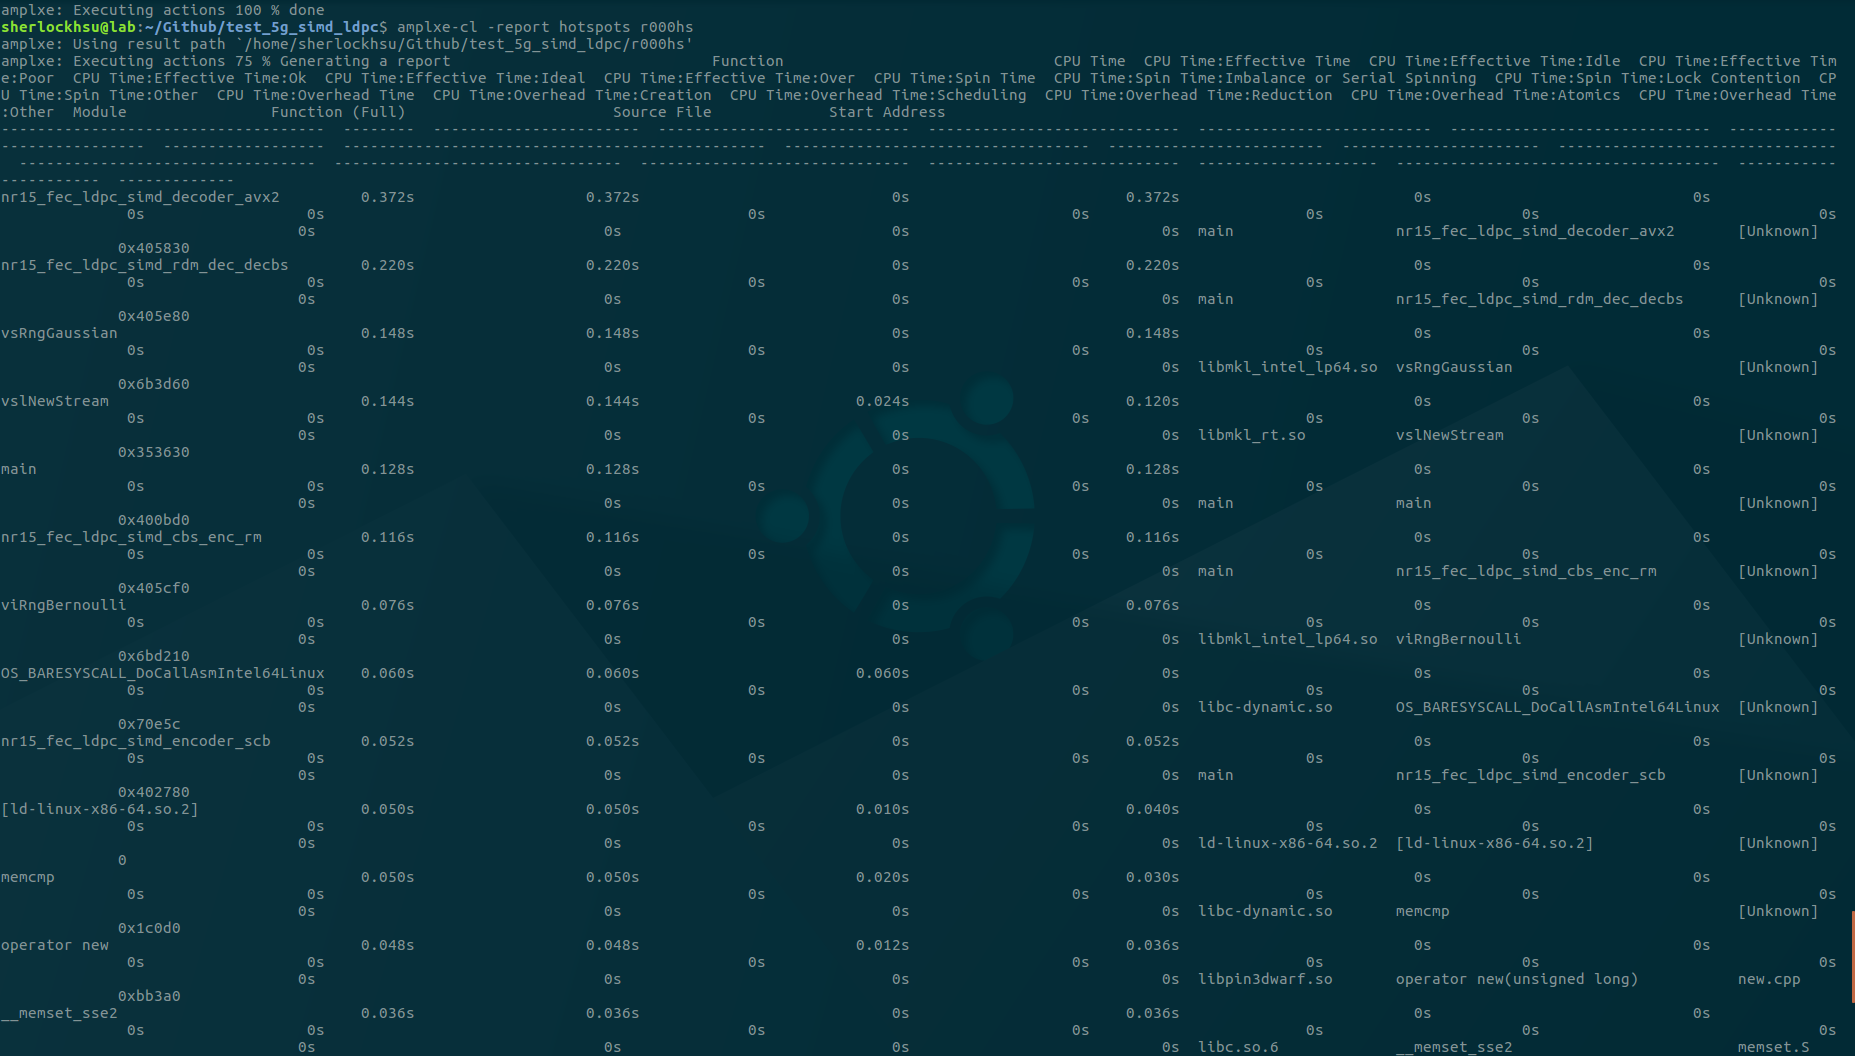
\includegraphics[width = \textwidth]{vtunel.png}
	\caption{本地VTune测试结果}
\end{figure}

\subsection{服务器测试}
\begin{figure}[H]
	\centering
	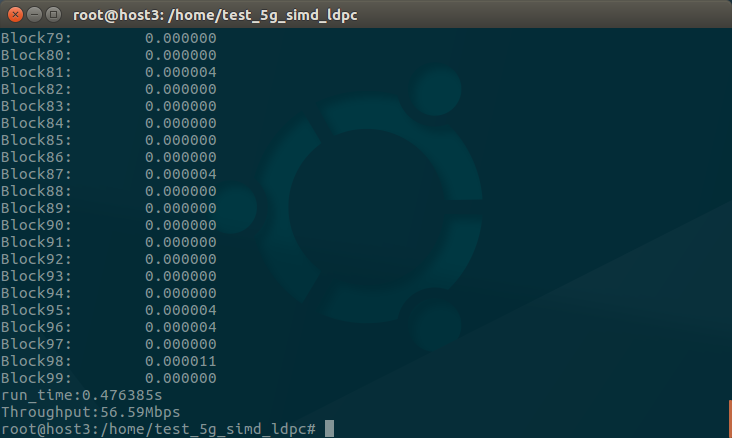
\includegraphics[width = .8\textwidth]{res.png}
	\caption{服务器运行结果}
\end{figure}
\begin{figure}[H]
	\centering
	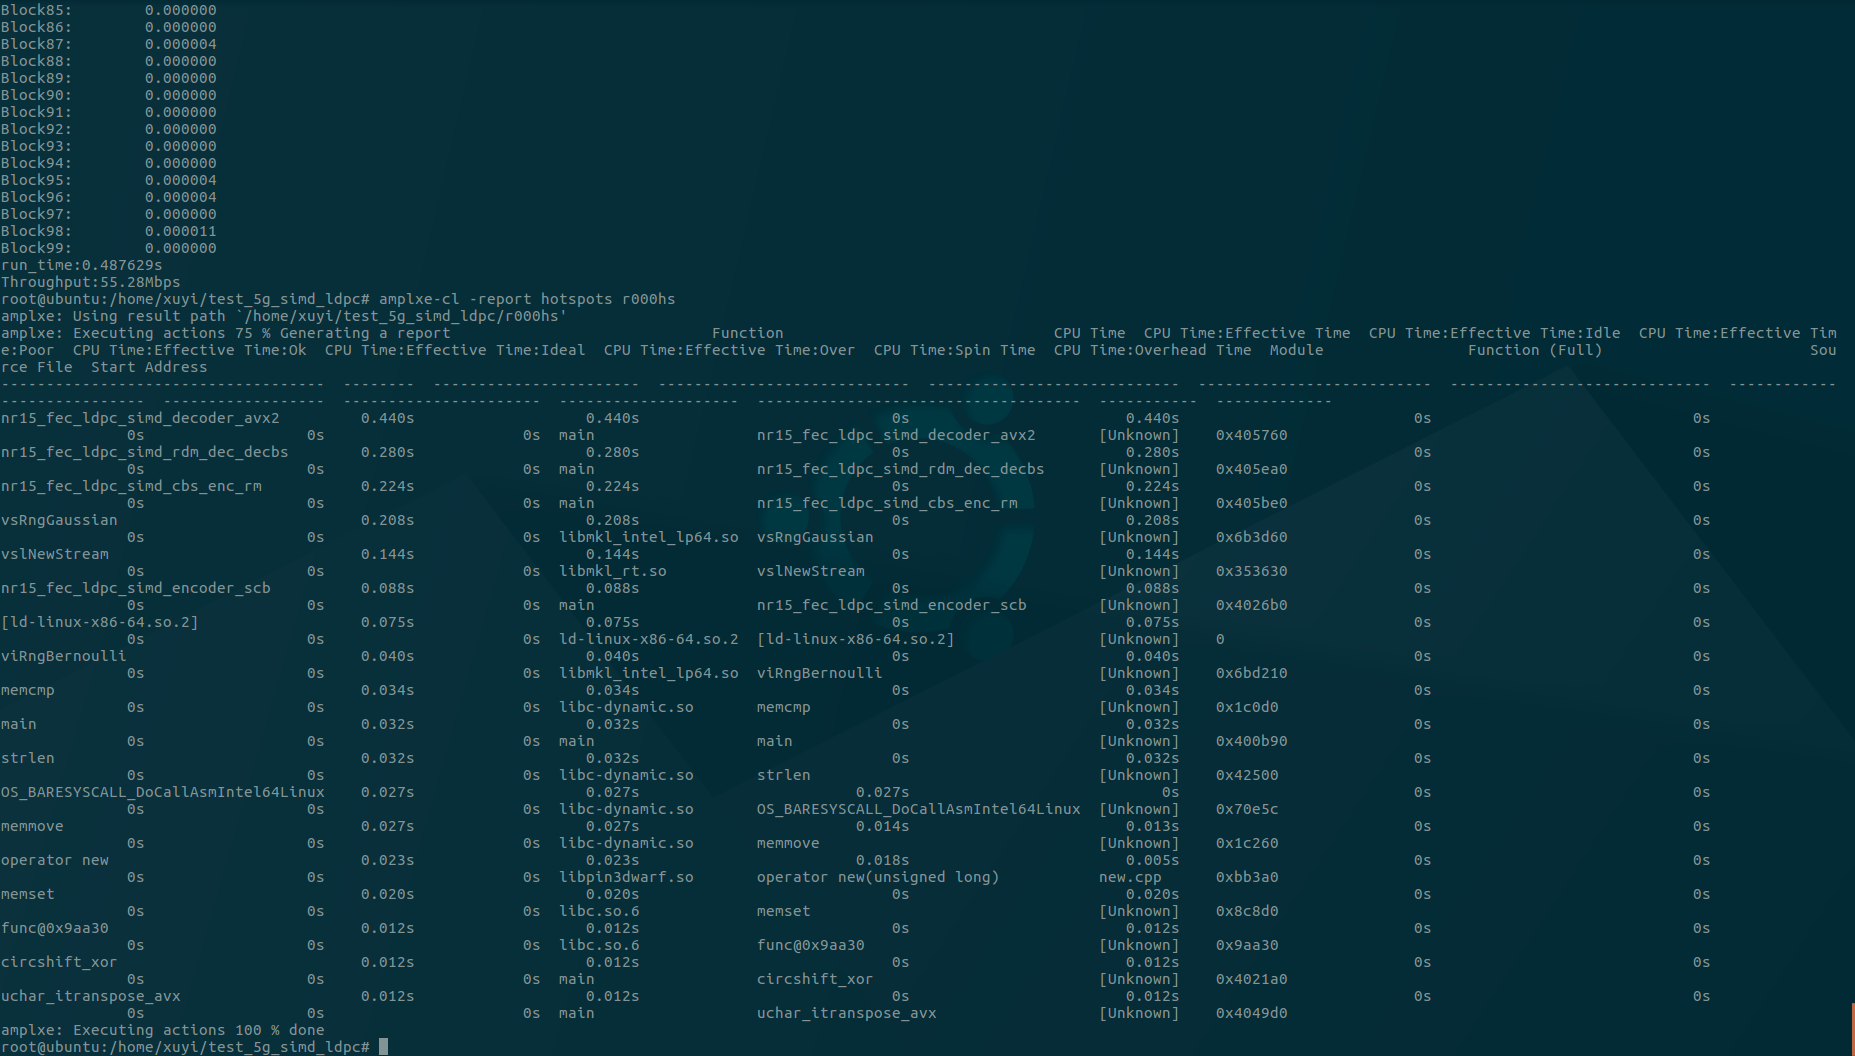
\includegraphics[width = \textwidth]{vtune.png}
	\caption{服务器VTune测试结果}
\end{figure}


%===========第四节=================
\section{仍存在的问题}


%===========下周计划=================
% \section{下阶段计划}
% 1. 进一步优化吞吐量性能

\end{document}
%%%%%%%%%%%%%%%%%%%%%%%这是正文部分的结束%%%%%%%%%%%%